\section{React Native}
\label{reactnative}

\subsection{Was ist React Native?}
React Native ist ein JavaScript-Framework, welches dafür verwendet wird, Cross-Platform-Apps für
die Betriebssysteme Android, iOS, Windows und MacOS zu entwickeln. Außerdem ist der Zugriff auf die
native Plattform-API möglich.

\subsection{Wie viel React steckt wirklich in React Native?}
Wie der Name schon vermuten lässt baut React Native hauptsächlich auf die JavaScript-Bibliothek
React auf. Sie hilft bei der Erstellung der Benutzeroberfläche, verwaltet den Zustand der
Anwendung und hat noch viele weitere kleine Aufgaben. React an sich ist noch eine Bibliothek,
mit -- absichtlich -- wenig "Grundgerüst". Das macht es auch für die Open-Source-Gemeinschaft
einfacher zusammen gute Lösungen zu entwickeln und so werden die wenigen wichtigen Aufgaben von
React dafür perfekt ausgeführt.
Detaillierte Informationen zu State, Render-Funktionen, Komponenten und JSX finden Sie im Kapitel
\nameref{reactjs}.

\subsection{Geschichte}
Die ersten Versionen der Facebook-App für Smartphones war eine Hybrid-App, also eine Webseite,
welche einfach in einer nativen App eingebunden wird \cite{reactNativeHistory}. Die Leistung der
Handy-App war für das Niveau des Social-Media-Giganten eindeutig zu schlecht, die App musste neu
geschrieben werden in Objective-C, womit Facebook sich eine 2,5-fach schnellere Anwendung erwartete
\cite{facebookNewIosApp}.

Nachdem React veröffentlicht worden war, versuchten die Entwickler bei Facebook einen effizienten
Weg zu finden, die neue Technologie zu nutzen um native Anwendungen, genauer eigentlich
Cross-Platform Anwendungen, zu schreiben.

2015 wurde die erste stabile Version von React Native veröffentlicht. Seit Anfang an verwendet
Facebook intern in ihren erfolgreichsten Apps React Native als Basistechnologie. Die Firma Microsoft
stellt selbst Bibliotheken zur Verfügung, um React Native Anwendungen auch für die Universal Windows
Platform (UWP) und MacOS zu entwickeln.

\subsection{Wer benutzt React Native?}
Laut der eigenen Webseite von React Native benutzen einige der größten Firmen der Welt React Native
als Cross-Platform-Framework für ihre Android- und iOS-Apps.

\begin{table}[H]
\centering
\begin{tabular}{|l|l|c|c|l|}
  \hline
  \textbf{Unternehmen} & \textbf{App} & \textbf{Android} & \multicolumn{1}{l|}{\textbf{iOS}} & \textbf{Bemerkung} \\ \hline\hline
  \multirow{5}{*}{Facebook} & Facebook             & \multicolumn{2}{c|}{\multirow{5}{*}{\XBox}} & \\
                            & Facebook Ads Manager & \multicolumn{2}{c|}{}                       & \\
                            & Facebook Analytics   & \multicolumn{2}{c|}{}                       & \\
                            & Instagram            & \multicolumn{2}{c|}{}                       & \\
                            & Oculus               & \multicolumn{2}{c|}{}                       & \\ \hline
  Microsoft                 & Skype                & \multicolumn{2}{c|}{\XBox}                  & \\ \hline
  Discord                   & Discord              & \Square          & \XBox                    & \\ \hline
  Tesla                     & Tesla                & \multicolumn{2}{c|}{\XBox}                  & \\ \hline
  Coinbase                  & Coinbase             & \multicolumn{2}{c|}{\XBox}                  & \\ \hline
  Walmart                   & Walmart              & \multicolumn{2}{c|}{\XBox}                  & \\ \hline
  Pinterest                 & Pinterest            & \multicolumn{2}{c|}{\XBox}                  & \\ \hline
  Uber                      & Uber Eats            & \multicolumn{2}{c|}{\XBox}                  & \\ \hline
  Shopify                   & Shopify              & \multicolumn{2}{c|}{\XBox}                  & \\ \hline
  Wix.com                   & Wix.com              & \multicolumn{2}{c|}{\XBox}                  & \\ \hline
\end{tabular}
\end{table}

\begin{center}
  Berühmte Beispiele für Apps mit React Native \cite{reactNativeShowcase}
\end{center}

\subsection{Lizenz}
React Native wird unter der MIT-Lizenz geführt, das heißt dass jeder die Software sowohl für
Open-Source als auch für Closed-Source-Projekte verwenden darf.

\section{Erstellung eines React Native Projekts}
Schon bei der Erstellung des Projekts müssen einige Fragen geklärt werden. Als erstes sollte man
sich wohl fragen, mit welcher CLI man das Projekt erstellen möchte.

Mit CLI (für engl. command-line-interface) ist in unserem Kontext eine Sammlung von Befehlen
gemeint, die in der Kommandozeile eines PCs ausgeführt werden können. Beispiele für Kommandozeilen-
Emulatoren:

\begin{itemize}
  \item Windows Powershell
  \item Windows Cmd
  \item MacOS zsh
  \item Git Bash
  \item Gnome Shell
\end{itemize}

\subsection{Expo CLI}
Die Entwickler von React Native selbst empfehlen allen Anfängern im Gebiet App-Entwicklung die
Verwendung der Expo CLI, welche eine vereinfachte Variante einer React Native Anwendung erzeugt.

Als Vorteil zählt auf jeden Fall die Geschwindigkeit, mit der eine neue App auf einem neuen Gerät
getestet werden kann. Dies ist meist innerhalb weniger Minuten möglich.

Ein wichtiger Nachteil ist jedoch, dass man in einem Expo-Projekt eingeschränkten Zugriff auf
Schnittstellen des Betriebssystems hat, es sind im Projekt nicht einmal die Ordner android und ios
vorhanden, um Änderungen vorzunehmen.

\subsubsection{Installation und Erstellung}
Um eine Expo React Native Anwendung erstellen zu können benötigt man als erstes \nameref{nodejs} und
den darin enthaltenen Node Package Manager. In einer Kommandozeile führt man nun folgende Befehle
aus, um die Expo-CLI im globalen Kontext zu installieren und anschließend ein Expo Projekt zu
erstellen. Nach der Auswahl für die Vorlage wir das Projekt erstellt.

\begin{lstlisting}
C:\example> npm install -g expo-cli
added 1549 packages, and audited 1550 packages in 1m

C:\example>expo init expoInitBlank
? Choose a template: - Use arrow-keys. Return to submit.
    ----- Managed workflow -----
>   blank               a minimal app as clean as an empty canvas
    blank (TypeScript)  same as blank but with TypeScript configuration
    tabs (TypeScript)   several example screens and tabs using react-navigation and TypeScript
    ----- Bare workflow -----
    minimal             bare and minimal, just the essentials to get you started
\end{lstlisting}

\subsubsection{Ordnerstruktur}
\begin{figure}[H]
  \begin{center}
    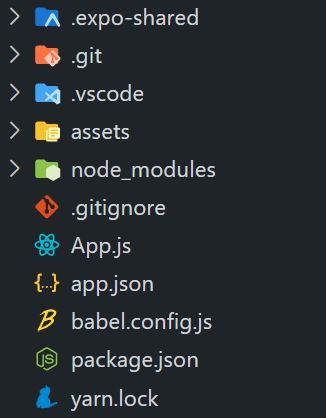
\includegraphics[width=0.5\textwidth]{Theorie/ReactNative/ExpoFolderStructure.JPG}
    \caption{Ordnerstruktur Expo Init Blank}
  \end{center}
\end{figure}

In den Ordnern .expo-shared, .git und .vscode befinden sich lediglich Konfigurationsdateien für Expo
selbst, die Versionsverwaltungssoftware Git und Visual Studio Code, dem Text-Editor, den wir
durchwegs für die gesamte Diplomarbeit verwendet haben.

Der Ordner assets ist für das Abspeichern von statischen Ressourcen, wie Bildern, Icons oder
ähnliches gedacht.

Im Ordner node\_modules werden alle Bibliotheken abgespeichert, die mit Hilfe des Paketmanagers
in das Projekt eingebunden wurden. Expo entschied sich gegen die Verwendung von NPM und verwendet
stattdessen Yarn.

Die wichtigste Datei im Projekt ist wohl App.js, sie stellt den Einstiegspunkt für das Projekt dar.

\begin{lstlisting}
import { StyleSheet, Text, View } from 'react-native';

function App() {
  return (
    <View style={styles.container}>
      <Text>Open up App.js to start working on your app!</Text>
    </View>
  );
}

const styles = StyleSheet.create({
  container: {
    flex: 1,
    backgroundColor: '#fff',
    alignItems: 'center',
    justifyContent: 'center',
  },
});

export default App;
\end{lstlisting}

In der ersten Zeile des Programms werden diverse React Native Core Components importiert. Core
Components sind, wörtlich übersetzt, die Kernkomponenten des Frameworks, mit ihnen wird der Großteil
der Benutzeroberfläche aufgebaut. Wie bereits erwähnt, werden die React Native Komponenten beim
Kompilieren in die richtigen Komponenten für das Zielsystem umgewandelt.

\begin{table}[H]
\centering
\begin{tabular}{|l|l|l|l|}
  \hline
  \textbf{Komponente} & \textbf{Android} & \textbf{iOS} & \textbf{HTML} \\ \hline\hline
  View                & ViewGroup        & UIView       & div          \\
  Text                & TextView         & UITextView   & p            \\ \hline
\end{tabular}
\end{table}

\begin{center}
  React Native Core Components und deren Äquivalente im Überblick \cite{reactNativeCoreComponents}
\end{center}

In der nächsten Zeile wird unserer erster React-Component erzeugt, welcher im Grunde nur eine
Funktion ist, die \nameref{jsx}-Code als Rückgabewert liefert.

In Zeile 5 wird zur View ein React Native StyleSheet zugewiesen. Man verwendet nämlich kein
gewöhnliches \nameref{css}, wie in der Webentwicklung, sondern ein relativ ähnlich aufgebautes,
eigenes System zur Gestaltung der App. Ein wichtiger Unterschied ist, dass die Attribut-Namen im
StyleSheet nicht durch Bindestriche getrennt, sondern in der LowerCamelCase-Notation geschrieben
werden \cite{camelCaseNotation}.

Am Ende der Datei wird noch die Komponente als Default exportiert, damit sie von Expo verarbeitet
werden kann \cite{jsModules}.

In die Datei .gitignore fügt man Datei- und Ordnernamen ein, die nicht von der Versionsverwaltung
gesichert werden sollen. Sehr zu empfehlen ist dies beim Ordner node\_modules, da dieser schon
direkt nach der Erstellung 170 Megabytes groß ist.

\subsection{}

\section{React Native CLI}
npx seit npm 5.2.0